\section{Menü-Struktur}

% Siehe auch: https://sopra.informatik.uni-freiburg.de/soprawiki/Men%C3%BC

% Bei der Beschreibung der Menü-Struktur wird erklärt, wie das Hauptmenü und
% alle In-Game-Menüs zueinander in Beziehung stehen. Hilfreich dazu kann ein
% Diagramm in Form eines Graphen oder Baums sein.
%
% Wichtig ist, dass ersichtlich wird, welche Aktion im Menü welche Reaktion des
% Interfaces verursacht. Beispiel: "Wenn man im Einstellungsmenü auf 'Zurück'
% klickt, gelangt man zurück ins Hauptmenü."
%
% Ebenso wichtig ist die Vollständigkeit der Beschreibung. Jedes Menü und jedes
% Untermenü sollten erklärt werden.

% \missingSection{Menü-Struktur}
Beim Starten von \textit{Kernel Panic!} öffnet sich nach der Hintergrundgeschichte direkt das \textit{Hauptmenü} (siehe Abbildung \ref{fig:menu}). Hier hat man Zugriff auf die \textit{Spielanleitung}, \textit{Statistiken}, \textit{Achievements} und die \textit{Credits}.\\
Das wählen einer dieser Felder öffnet ein Fenster, in dem man diverse Informationen zum entsprechenden Thema einsehen kann. Mithilfe des Feldes \textit{Zurück} oder dem Betätigen der \textit{Escape}-Taste gelangt man wieder in das Hauptmenü.\\
Um das Spiel zu beenden wählt man im Hauptmenü das Feld \textit{Beenden}. Damit man nicht versehentlich das Spiel schließt öffnet sich zunächst noch ein zusätzliches Fenster, man kann nun entweder das Beenden bestätigen oder zurückkehren.\\
Das Feld \textit{Spielen} öffnet das Menü, dass für das Erstellen beziehungsweise das Laden des Spieles zuständig ist. Wenn man nicht durch Wählen der Escape-Taste oder Betätigen des \textit{Zurück}-Feldes das Hauptmenü öffnet, wählt man hier einen von fünf Spielständen, sogenannten \textit{Spielslots}. Jeder \textit{Spielslot} kann entweder genau einen zuvor gespeicherten Spielstand enthalten oder \textit{leer} sein.\\
Wenn man einen nicht-\textit{leeren} \textit{Spielslot} ausgewählt hat kann man ein angefangenes \textit{Spiel laden} oder ein \textit{Spiel erstellen}; falls der aktuelle \textit{Spielslot} \textit{leer} ist bleibt nur die Option ein neues \textit{Spiel} zu \textit{erstellen}.\\
Unabhängig davon ob der \textit{Spielslot} frei ist, gelangt man nun in das Spiel.\\
Während dem Spiel kann man zu jedem Zeitpunkt pausieren - es öffnet sich das \textit{Pause}-Menü.\\
Hier gibt es unter anderem die beiden Felder \textit{Speichern} und \textit{Laden}.\\
\textit{Speichern} ersetzt den gesicherten Spielstand des aktuellen \textit{Spielslots} durch eine Kopie des aktuellen Spiels zu diesem Zeitpunkt.\\
\textit{Spiel Laden} ersetzt das aktuell pausierte Spiel durch das zuvor gesicherte. Innerhalb des Spiels kann weder durch \textit{Spiel speichern}, noch \textit{Spiel laden} den \textit{Spielslot} wechseln, dafür müsste man zunächst in das \textit{Hauptmenü}, welches mithilfe des Feldes \textit{Hauptmenü} erreicht werden kann.\\
Es gibt noch ein weiteres Menü: die \textit{Optionen}, diese lassen sich durch wählen des Feldes \textit{Optionen} sowohl aus dem \textit{Hauptmenü} als auch direkt aus dem \textit{pausierten} Spiel öffnen. Dementsprechend führt auch das \textit{Zurück} Feld, beziehungsweise die \textit{Escape}-Taste wieder zum vorherigen Menü.\\
Es lassen sich hier nun verschiedene Audio-Einstellungen treffen. Soundeffekte und Musik können über je ein eigenes Feld stummgeschalten werden. Außerdem hat man die Möglichkeit über einen Schieberegler die Lautstärke der jeweiligen Komponente einzustellen.\\
Auch die Tastaturbelegung wird im Menü \textit{Optionen} angepasst. Es gibt für alle individualisierbare Aktionen die Möglichkeit die Standartbelegung zu ändern oder eine alternative Taste festzulegen.\\
Man wählt hierfür das zu ändernde Feld aus und überschreibt die gespeicherte Taste mit dem nächsten Input.

\begin{figure}[ht]
	\centering
	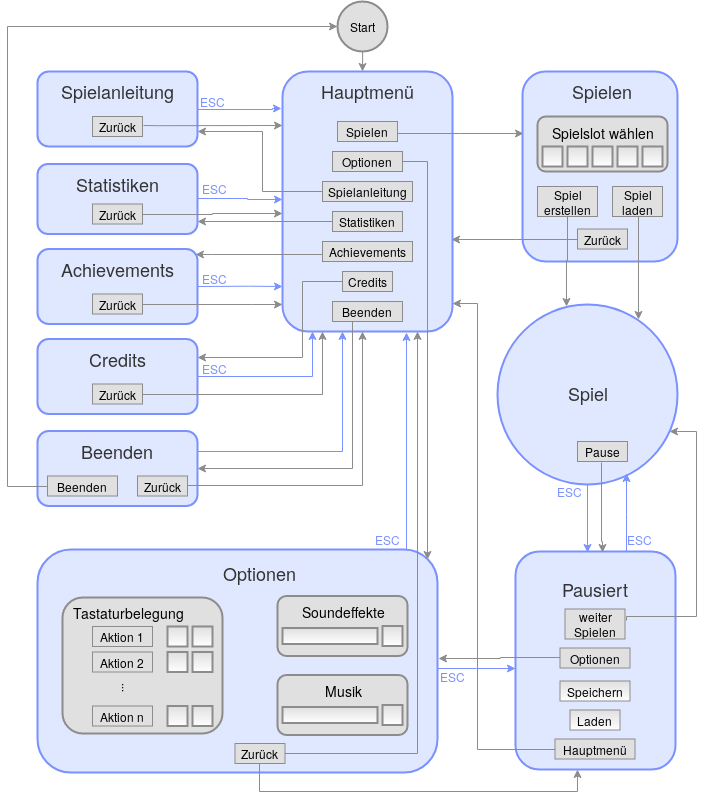
\includegraphics[width=1\textwidth]{menu_structure.png}
	\caption{Menü-Struktur}
	\label{fig:menu}
\end{figure}


% 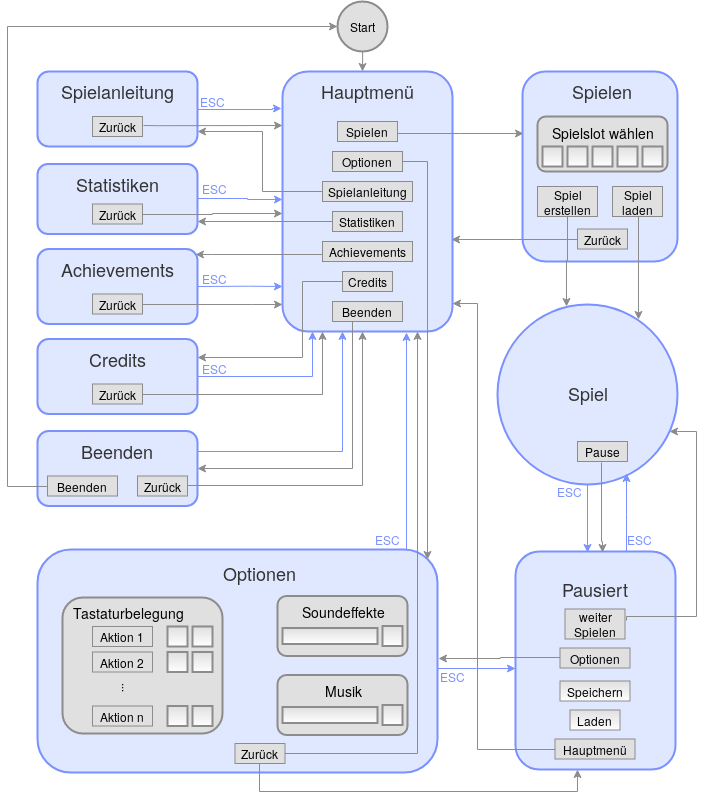
\includegraphics[width=\textwidth]{menu_structure.png}